%++++++++++++++++++++++++++++++++++++++++
% Don't modify this section unless you know what you're doing!
%\documentclass[letterpaper,12pt]{article}
\documentclass[a4paper]{article}
\usepackage{tabularx} % extra features for tabular environment
\usepackage{amsmath}  % improve math presentation
\usepackage{graphicx} % takes care of graphic including machinery
%\usepackage[margin=1in,letterpaper]{geometry} % decreases margins
\usepackage{cite} % takes care of citations
%\usepackage[final]{hyperref} % adds hyper links inside the generated pdf file
%\hypersetup{
%	colorlinks=true,       % false: boxed links; true: colored links
%	linkcolor=blue,        % color of internal links
%	citecolor=blue,        % color of links to bibliography
%	filecolor=magenta,     % color of file links
%	urlcolor=blue
%}
%++++++++++++++++++++++++++++++++++++++++
\usepackage{indentfirst}
\usepackage{tensor}
\usepackage{amssymb}
\allowdisplaybreaks
\usepackage{bm}
\newcommand{\at}[2][]{#1|_{#2}}
\newcommand\numberthis{\addtocounter{equation}{1}\tag{\theequation}}
\newcommand\norm[1]{\left\lVert#1\right\rVert}

\usepackage[none]{hyphenat} % Avoids to go out of margin

% Fontsize of figure smaller than normalsize:
\usepackage{caption}
\captionsetup[figure]{font=small}
\captionsetup[table]{font=small}

%\usepackage{setspace} % doublespacing
\linespread{1.2}

\begin{document}
\sloppy % Avoids to go out of margin

%\title{Torso Pose Estimation on the\\HRP4 Humanoid Robot\\(draft)}
%\author{Michele Cipriano, Godwin Joey, Lorenzo Vianello\\Supervised by Nicola Scianca}
%\date{\today}
%\maketitle

\title{FP2\\Torso Pose Estimation on the HRP4 Humanoid Robot}								% Title
\author{Michele Cipriano, Godwin K. Peprah, Lorenzo Vianello\\Supervised by Nicola Scianca}								% Author
\date{\today}											% Date

\makeatletter
\let\thetitle\@title
\let\theauthor\@author
\let\thedate\@date
\makeatother

\begin{titlepage}
	\centering
    \vspace*{0.5 cm}
    
\includegraphics[scale = 0.75]{images/SapienzaLogo}\\[1.0 cm]	% University Logo

    \vspace*{-0.4cm}
    \textsc{\large Department of Computer, Control and\\Management Engineering}\\[2.0 cm]	% Department Name
    \vspace*{1cm}

    { \fontsize{20.74pt}{18.5pt}\selectfont\bfseries \thetitle \par } % title

    \vspace*{0.1cm}
    \textsc{\Large Autonomous and Mobile Robotics\\Robotics 2}\\[0.5 cm] % course name

    \vspace*{2.6cm}
	\begin{minipage}{0.4\textwidth}
		\begin{flushleft} \large
			\emph{Professors:}\\
			Giuseppe Oriolo\\
            Alessandro De Luca\\
            %Computer Science Department\\
		\end{flushleft}
	\end{minipage}~
	\begin{minipage}{0.4\textwidth}
		\begin{flushright} \large
			\emph{Students:} \\
			Michele Cipriano\\
            Godwin K. Peprah\\
            Lorenzo Vianello\\
            \vspace*{0.2cm}
            \emph{Supervisor:}\\
			Nicola Scianca
            %Semester\\
		\end{flushright}

	\end{minipage}\\[2 cm]

    \vspace{0.2cm}
    \rule{\linewidth}{0.2 mm} \\[0.3 cm]
    \vspace*{-0.3cm}
    Academic Year 2017/2018
\end{titlepage}

\tableofcontents
\newpage

%\begin{abstract}
%In this experiment we studied a very important physical effect by measuring the
%dependence of a quantity $V$ of the quantity $X$ for two different sample
%temperatures.  Our experimental measurements confirmed the quadratic dependence
%$V = kX^2$ predicted by Someone's first law. The value of the %mystery parameter
%$k = 15.4\pm 0.5$~s was extracted from the fit. This value is
%not consistent with the theoretically predicted $k_{theory}=17.34$~s. We attribute this
%discrepancy to low efficiency of our $V$-detector.
%\end{abstract}

%\begin{abstract}
%Todo.
%\end{abstract}

\section{Introduction}

The aim of the project is the estimate the pose of the torso on the HRP4
humanoid robot following the methodologies introduced in
\cite{DBLP:journals/arobots/OrioloPRV16}. Knowing the pose of the torso is
extremely important because it can be used to localize any other point of
the robot using kinematic computations based on joint encoder readings.
The idea is to use this estimate in order to obtain the position of the CoM %/ZMP
of the robot so that it can be used to close the feedback loop in the
MPC gait generator.

In our approach, we have developed an Extended Kalman Filter (EKF) to estimate
the pose of the torso, using
the joint encoders, the Inertial Measurement Unit (IMU) and a RGBD camera
as sensors. We first used only the accelerometer and the gyroscope of the IMU
as measurements, obtaining good results on the estimate of the orientation but
diverging results on the position. We then improved the EKF by filtering the
linear velocities of the torso (previously obtained by integrating the linear
acceleration read by the accelerometer sensor) obtaining convergence on the
$x$, $y$ axes and reducing the error on the $z$ axis. The introduction of the
RGBD camera, less susceptible to noise and drift, further improved the
estimate of the position of the torso, obtaining convergence on the $z$
axis as well. In this last step we used the trilateration algorithm.

We tested the behaviour of the EKF by modeling the robot as a unicycle
in order to make it perform a cartesian and a posture regulation task,
correctly achieving the desired final configuration in both cases.

In the end, we tried to close the feedback loop in the
MPC gait generator obtaining unsuccessful results.

The project has been entirely developed in C++ using the HRP4 humanoid robot
model in a V-REP environment.

\section{Torso Pose Estimation}
This section introduces the kinematic model used for the Extended Kalman Filter,
describing in details its whole implementation and the different methods used
to provide the measurements to the filter itself.

\subsection{Kinematic Model}
Let $\bm{x} = (\bm{p}_t^T, \bm{o}_t^T)^T$ be the pose of the torso frame $\mathcal{F}_t$
with respect to the world frame $\mathcal{F}_w$. We want to
develop a filter that estimates the state $\bm{x}$ while
it moves around the environment. Let $\mathcal{F}_s$ be the
support foot frame with respect to the world frame and let
$\bm{o}_s$ be its orientation.
Let $\bm{J}(\bm{q}_s, \bm{o}_s)$ the Jacobian
matrix of the kinematic map from the support frame
$\mathcal{F}_s$ to the torso frame $\mathcal{F}_t$.
Let's use the following kinematic model to describe the
evolution of the state $\bm{x}$ through time:
\begin{equation}
    \bm{\dot{x}} = \bm{J}(\bm{q}_s, \bm{o}_s) \bm{\dot{q}}_s
    \label{eq:hrp4-kinematic-model}
\end{equation}

\noindent with $\bm{\dot{q}}_s$ velocities of the support joints
acting as control inputs. Note that the Jacobian
$\bm{J}(\bm{q}_{s}, \bm{o}_s)$ does not depend on the
position of $\mathcal{F}_s$:
\begin{align*}
    \bm{f}(\bm{q}_s, \bm{o}_s) &= \bm{\varOmega} \left(
        \begin{bmatrix}
            \bm{R}_z(\bm{o}_s) & \bm{0} \\
            \bm{0}^T & 1
        \end{bmatrix}
        \bm{\varOmega}^{-1}\left(
        \begin{bmatrix}
             \tensor[^s]{\bm{p}}{_t} \\
             \tensor[^s]{\bm{o}}{_t}
        \end{bmatrix}
        \right)
        \right) \\
%        &= \bm{\varOmega} \left(
%        \begin{bmatrix}
%            \bm{R}_z(\bm{o}_s) & \bm{0} \\
%            \bm{0}^T & 1
%        \end{bmatrix}
%         \begin{bmatrix}
%            \tensor[^s]{\bm{R}}{_t}(\tensor[^s]{\bm{o}}{_t}) & \tensor[^s]{\bm{p}}{_t} \\
%            \bm{0}^T & 1
%        \end{bmatrix}
%        \right) \\
%        &= \bm{\varOmega} \left(
%        \begin{bmatrix}
%            \bm{R}_z(\bm{o}_s) \tensor[^s]{\bm{R}}{_t}(\tensor[^s]{\bm{o}}{_t}) & \bm{R}_z(o_s) \tensor[^s]{\bm{p}}{_t}  \\
%            \bm{0}^T & 1
%        \end{bmatrix}
%        \right) \\
%        &= \bm{\varOmega} \left(
%        \begin{bmatrix}
%            \bm{R}_z(\bm{o}_s) \bm{R}_z(\tensor[^s]{\bm{o}}{_{t,z}}) \bm{R}_y(\tensor[^s]{\bm{o}}{_{t,y}}) \bm{R}_x(\tensor[^s]{\bm{o}}{_{t,x}}) & \bm{R}_z(o_s) \tensor[^s]{\bm{p}}{_t}  \\
%            \bm{0}^T & 1
%        \end{bmatrix}
%        \right) \\
        &= \bm{\varOmega} \left(
        \begin{bmatrix}
            \bm{R}_z(\bm{o}_s + \tensor[^s]{\bm{o}}{_{t,z}}) \bm{R}_y(\tensor[^s]{\bm{o}}{_{t,y}}) \bm{R}_x(\tensor[^s]{\bm{o}}{_{t,x}}) & \bm{R}_z(\bm{o}_s) \tensor[^s]{\bm{p}}{_t}  \\
            \bm{0}^T & 1
        \end{bmatrix}
        \right) \numberthis \\
%        &=
%        \begin{pmatrix}
%            \bm{R}_z(\bm{o}_s) \tensor[^s]{\bm{p}}{_t} \\
%            \tensor[^s]{\bm{o}}{_{t,x}} \\
%            \tensor[^s]{\bm{o}}{_{t,y}} \\
%            \bm{o}_s + \tensor[^s]{\bm{o}}{_{t,z}}
%        \end{pmatrix} \\
%        &=
%        \begin{bmatrix}
%            \bm{R}_z(\bm{o}_s) & \bm{O} \\
%            \bm{O} & \bm{I}
%        \end{bmatrix}
%        \begin{pmatrix}
%            \tensor[^s]{\bm{p}}{_t} \\
%            \tensor[^s]{\bm{o}}{_t}
%        \end{pmatrix}
%        +
%        \begin{pmatrix}
%            \bm{0}_{5} \\
%            \bm{o}_s
%        \end{pmatrix} \\
        &=
        \begin{bmatrix}
            \bm{R}_z(\bm{o}_s) & \bm{O} \\
            \bm{O} & \bm{I}
        \end{bmatrix}
        \bm{f}(\bm{q}_s)
        +
        \begin{pmatrix}
            \bm{0}_{5} \\
            \bm{o}_s
        \end{pmatrix} \\
    \bm{J}(\bm{q}_s, \bm{o}_s) &= \frac{\partial \bm{f}(\bm{q}_s, \bm{o}_s)}{\partial \bm{q}_s} \\
    &=
    \begin{bmatrix}
            \bm{R}_z(\bm{o}_s) & \bm{O} \\
            \bm{O} & \bm{I}
    \end{bmatrix}
    \frac{\partial \bm{f}(\bm{q}_s)}{\partial \bm{q}_s} \numberthis \\
    &=
    \begin{bmatrix}
            \bm{R}_z(\bm{o}_s) & \bm{O} \\
            \bm{O} & \bm{I}
    \end{bmatrix}
    \bm{J}(\bm{q}_s)
\end{align*}

\noindent which definition is important for development purposes.
In fact, $\bm{J}(\bm{q}_s)$ is easily accessible thanks to the
C++ implementation of the HRP4 kinematics. Note that, unless
specified otherwise, $\bm{I} \in \mathbb{R}^{3 \times 3}$
represents the identity matrix,
$\bm{O} \in \mathbb{R}^{3 \times 3}$
represents the zero matrix, while $\bm{0} \in \mathbb{R}^{3}$
represents the zero vector. $\bm{\varOmega}$ is a function that
returns a minimal representation of a transform function.
% NOTE: it is not an Eigen function
%In the C++ library \texttt{Eigen}, $\bm{\varOmega}$ is
%implemented
%with \texttt{t2v}, while $\bm{\varOmega}^{-1}$ is implemented
%with \texttt{v2t}.

The robot is equipped with a RGBD camera and an IMU, used
to measure the pose of the torso frame:
\begin{equation}
\label{eq:ekf-observation-function}
    \bm{y} = \bm{h}(\bm{x}, \bm{q}_n) =
        \begin{pmatrix}
            \bm{p}_t \\
            \bm{o}_t
        \end{pmatrix}
\end{equation}

In particular, the position $\bm{p}_t$ is computed by doing either
trilateration exploiting known position of the landmarks or integrating the
data coming from the accelerometer, while
the orientation $\bm{o}_t$ is computed by simply integrating
the data obtained from the gyroscope. The measurements of the pose of the
torso $\bm{y}$ depend on the estimation of the pose of the torso $\bm{x}$ and the
configuration of the neck joints $\bm{q}_n$. Details are explained in
subsections \ref{subsec:accelerometer-integration}--\ref{subsec:trilateration}.
Note that the notation $\bm{q}_s$ and $\bm{q}_n$ have been kept in order to
be consistent with the main reference paper but are not actually used in
the implementation. The whole configuration of the robot $\bm{q}$ is used instead.

\subsection{Extended Kalman Filter}
\label{subsec:ekf}
It is now possible to define a discrete-time stochastic system
using Equations \ref{eq:hrp4-kinematic-model}-\ref{eq:ekf-observation-function},
with $T$ sampling
interval of the filter and $k$ current timestep:
\begin{align}
    \bm{x}_{k+1} &= \bm{x}_k + T \bm{J}(\bm{q}_{s,k}, \bm{o}_s) \bm{\dot{q}}_{s,k} + \bm{v}_k \\
    \bm{y}_k &= \bm{h}(\bm{x}_k, \bm{q}_{n,k}) + \bm{w}_k
\end{align}

\noindent with $\bm{v}_k \sim \bm{\mathcal{N}}(\bm{0}, \bm{V}_k)$ and $\bm{w}_k \sim \bm{\mathcal{N}}(\bm{0}, \bm{W}_k)$ zero-mean
white Gaussian noises and
$\bm{V}_k \in \mathbb{R}^{6 \times 6}$,
$\bm{W}_k \in \mathbb{R}^{6 \times 6}$ their respective
covariance matrices.

%%% EKF Prediction.

At each timestep, a prediction $\bm{\hat{x}}_{k+1|k}$ is
generated using the current estimate $\bm{\hat{x}}_{k}$:
\begin{equation}
    \bm{\hat{x}}_{k+1|k} = \bm{\hat{x}}_k + \bm{J}(\bm{q}_{s,k}, \bm{o}_s) \Delta \bm{q}_{s,k},
    \quad \Delta \bm{q}_{s,k} = \bm{q}_{s,k+1} - \bm{q}_{s,k}
\end{equation}

\noindent with $\Delta \bm{q}_{s,k} \approx T \bm{\dot{q}}_{s,k}$
obtained using encoder readings. The covariance prediction
matrix is updated accordingly:
\begin{equation}
    \bm{P}_{k+1|k} = \bm{P}_{k} + \bm{V}_{k}
\end{equation}

In the same way as before, the predicted output
associated to $\bm{\hat{x}}_{k+1|k}$ is computed as well:
\begin{equation}
    \bm{\hat{y}}_{k+1|k} = \bm{h}(\bm{\hat{x}}_{k+1|k}, \bm{q}_{n, k+1})
\end{equation}

%%% EKF Correction.
To correct the predicted state we need to compute the
innovation using the measurements and the predicted
output computed in the previous step:
\begin{equation}
    \bm{\nu}_{k+1} = \bm{y}_{k+1} - \bm{\hat{y}}_{k+1|k}
\end{equation}

It is, hence, possible to determine the corrected state
estimate by computing:
\begin{equation}
    \bm{\hat{x}}_{k+1} = \bm{\hat{x}}_{k+1|k} + \bm{G}_{k+1} \bm{\nu}_{k+1}
\end{equation}

\noindent with $\bm{G}_{k+1}$ Kalman gain matrix, defined as
\begin{align}
    \bm{G}_{k+1} &= \bm{P}_{k+1|k} \bm{H}_{k+1}^T \left( \bm{H}_{k+1} \bm{P}_{k+1|k} \bm{H}_{k+1}^T + \bm{W}_{k+1} \right)^{-1} \\
        &= \bm{P}_{k+1|k} (\bm{P}_{k+1|k} + \bm{W}_{k+1})^{-1}
\end{align}

\noindent since the partial derivative of the observation
function with respect to the state is the identity matrix:
\begin{align}
    \bm{H}_{k+1} = \frac{\partial \bm{h}}{\partial \bm{x}} \at[\bigg]{\bm{x}=\bm{\hat{x}}_{k+1|k}}
        = \bm{I}
\end{align}

The corrected covariance matrix is updated as well:
\begin{align}
    \bm{P}_{k+1} &= \bm{P}_{k+1|k} - \bm{G}_{k+1} \bm{H}_{k+1} \bm{P}_{k+1|k} \\
        &= \bm{P}_{k+1|k} - \bm{G}_{k+1} \bm{P}_{k+1|k}
\end{align}

Note that, in our implementation, we defined the covariance
matrices $\bm{V}$ and $\bm{W}$ as:
\begin{align}
    \bm{V} &= \text{diag}\{5, 5, 5, 100, 100, 100 \} \cdot 10^{-6} \\
    \bm{W} &= \text{diag}\{5, 5, 5, 5 \cdot 10^{-2}, 5 \cdot 10^{-2}, 5 \cdot 10^{-2} \}  \cdot 10^{-2}
\end{align}

\subsection{Accelerometer Integration}
\label{subsec:accelerometer-integration}

As said before, the measurement of the position of the torso $\bm{p}_t$ can be computed
by either doing trilateration, exploiting the known position of the landmarks, or
by integrating the data coming from the accelerometer. Let's discuss the second
approach considering constant acceleration $\bm{\ddot{p}}_{t, k}$ in an interval $[t_k, t_{k+1})$:
\begin{align}
    \label{eq:velocity-accelerometer-integration}
    \bm{\dot{p}}_{t, k+1} &= \bm{\dot{p}}_{t, k} + \bm{\ddot{p}}_{t, k} T \\
    \label{eq:position-accelerometer-integration}
    \bm{p}_{t, k+1} &= \bm{p}_{t, k} + \bm{\dot{p}}_{t, k} T + \frac{1}{2} \bm{\ddot{p}}_{t, k} T^2
\end{align}

Note that the implementation of the accelerometer returns, at each timestep $k$,
the linear acceleration $\tensor[^t]{\bm{a}}{_{t,k}}$ expressed in the
current reference frame of the torso, hence, it must be transformed to the
reference frame of the world in order be able to perform the integration:
\begin{equation}
    \bm{\ddot{p}}_{t,k} = \tensor[^w]{\bm{R}}{_t}(\bm{\hat{x}}_{k}) \tensor[^t]{\bm{a}}{_{t,k}} - \bm{g}
\end{equation}

\noindent with $\bm{g} = [0, 0, -g]^T, g = 9.81 \text{m/s}^2$ and with:
\begin{equation}
    \tensor[^w]{\bm{R}}{_t}(\bm{\hat{x}}_{k}) = \bm{R}_z(\gamma) \bm{R}_y(\beta) \bm{R}_x(\alpha)
\end{equation}

\noindent where $\alpha$, $\beta$ and $\gamma$ are, respectively,
the roll, the pitch and the yaw angles of $\bm{\hat{x}}_{k}$.

\subsection{Gyroscope Integration}
\label{subsec:gyro-integration}
In a similar way, the gyroscope data can be integrated to obtain the
orientation of the robot $\bm{o}_t$ at each timestep. Considering a constant angular
velocity in an interval $[t_k, t_{k+1})$:
\begin{equation}
    \label{eq:orientation-gyro-integration}
    \bm{o}_{t,k+1} = \bm{o}_{t,k} + T \bm{\dot{o}}_{t,k}
\end{equation}

%Gyroscope integration (Trapezoidal).
%\begin{equation}
%    \bm{o}_{t,k+1} = \bm{o}_{t,k} + T \frac{\bm{\dot{o}}_{t,k} + \bm{\dot{o}}_{t,k-1}}{2}
%\end{equation}

Note that the implementation of the gyroscope returns, at each
timestep $k$, the angular velocity
$\tensor[^t]{\bm{\omega}}{_{t,k}}$ expressed in the current
reference frame of the torso, hence, it must be related to $\bm{\dot{o}}_{t,k}$
in order to be able to perform the integration:
\begin{equation}
    \bm{\dot{o}}_{t,k} = \bm{T}(\bm{\hat{x}}_{k}) \tensor[^t]{\bm{\omega}}{_{t,k}}
\end{equation}

\noindent with \cite{DBLP:conf/smc/LeeBDSXT09}:
\begin{equation}
    \bm{T}(\bm{\hat{x}}_{k}) =
    \begin{pmatrix}
        1 & \text{sin}(\alpha) \text{tan}(\beta) & \text{cos}(\alpha) \text{tan}(\beta) \\
		0 & \text{cos}(\alpha) & -\text{sin}(\alpha) \\
		0 & \text{sin}(\alpha)/\text{cos}(\beta) & \text{cos}(\alpha)/\text{cos}(\beta)
    \end{pmatrix}
\end{equation}

%\begin{equation}
%    \bm{\dot{o}}_{t,k} = [\tensor[]{\bm{T}}{_{RPY}}(\bm{\hat{x}}_{k})]^{-1} \tensor[^t]{\bm{\dot{o}}}{_{t,k}}
%\end{equation}

%\noindent with:
%\begin{equation}
%    \tensor[]{\bm{T}}{_{RPY}}(\bm{\hat{x}}_{k}) =
%    \begin{pmatrix}
%        \text{cos}(\beta) \text{cos}(\gamma) & -\text{sin}(\gamma) & 0 \\
%        \text{cos}(\beta) \text{sin}(\gamma) &  \text{cos}(\gamma) & 0 \\
%        -\text{sin}(\beta) & 0 & 1
%    \end{pmatrix}
%\end{equation}

\noindent where $\alpha$ and $\beta$ are, respectively,
the roll and the pitch angles of $\bm{\hat{x}}_{k}$.
%\noindent where $\tensor[^w]{\bm{R}}{_t}(\bm{\hat{x}}_{k+1|k})$ represents
%the rotation matrix
%from the reference frame of the torso to the reference frame
%of the world (roll-pitch-yaw angles determined by the %estimate
%$\bm{\hat{x}}_{k+1|k}$).%, while $\tensor[^t]{\bm{\dot{o}}}{_{t,k}}$
%represents the angular velocity of the torso expressed in the
%reference frame of the torso at time $k$.

\subsection{Trilateration}
\label{subsec:trilateration}
Let's now discuss how
trilateration\cite{trilateration-hereman-1995} can be used with
a RGBD camera in order to obtain the position of the torso
$\bm{p}_t$. We will find the position $\bm{p}_h$ of the camera
in order to obtain the position of the torso.

First, it's important to have landmarks that can be
easily recognizable. To achieve this, we have added to the scene
$n=6$ spheres of different colors. The camera of the robot is
pointing towards the
sky in order to simplify the recognition of the spheres
themselves avoiding the colors of the terrain.
Moreover, the specular, the emissive and the auxiliary
components of the spheres are the same as their ambient component
in order to avoid shades. This allows to have pixels of the same
color when seeing a sphere. It is, hence, possible to obtain
the pixel coordinates $(p_x, p_y)^T$ of each sphere in the image
of the camera by computing the centroid (a simple weighted mean
in our implementation) of the sphere itself.

Let $w$ and $h$ be the width and the
height of the images coming from the RGB camera. Let $\lambda$ be
the focal length (length to the nearest clipping
plane), $\lambda_f$ be the length to the furthest clipping plane and
$\phi$ be the perspective angle of the camera. It is possible
to obtain the position (expressed with respect to
the reference frame of the camera) of each sphere with centroid
at coordinates $(p_x, p_y)^T$ by simply considering the proportion
between the ratio of the pixel coordinates (translated so
that the origin is at $(0, 0)^T$) and half the size of the
image (in particular width when computing the $x$ component,
height when computing the $y$ component), and the ratio between
the coordinates of the sphere (in camera frame) and the distance
between the considered point with the axes $x$ and $y$ of the
camera frame. This results in a simple computation:
\begin{align}
    \tensor[^{cam}]{x}{} = \frac{2 p_x - w}{w} \tensor[^{cam}]{z}{} \cdot tan\left(\frac{\phi}{2}\right) \\
    \tensor[^{cam}]{y}{} = \frac{2 p_y - h}{h} \tensor[^{cam}]{z}{} \cdot tan\left(\frac{\phi}{2}\right)
\end{align}

\noindent with $(\tensor[^{cam}]{x}{}, \tensor[^{cam}]{y}{},
\tensor[^{cam}]{z}{})^T$ coordinates of the considered point
in the camera frame. Note that $\tensor[^{cam}]{z}{}$ can be
computed by
considering the distance from the clipping planes and the
depth $p_z$ of the object at position $(p_x, p_y)^T$, which can
be obtained by using the depth sensor of the RGBD camera:
\begin{equation}
    \tensor[^{cam}]{z}{} = (\lambda_f - \lambda) \cdot p_z + \lambda
\end{equation}

Moreover, note that the depth sensor returns a value between $0$ and $1$.
In particular, it returns $0$ if a point is exactly
on the nearest clipping plane, $1$ if a point is exactly on the
furthest clipping plane.

Given that each sphere has radius $\bar{r}$, it is possible to
obtain the distance from the camera to each sphere $i$ by computing:
\begin{equation}
    r_i =
    \norm{
        \begin{pmatrix}
            \tensor[^{cam}]{x}{_i} \\
            \tensor[^{cam}]{y}{_i} \\
            \tensor[^{cam}]{z}{_i}
        \end{pmatrix}
    }^2 + \bar{r} \quad (i = 1, 2, \dots, n)
\end{equation}

\noindent where the subscript $i$ specifies the index of the
sphere. Note that adding $\bar{r}$ to the norm is an
approximation of the real distance since the centroid could
not be along the line passing through the position of the
camera and the center of the sphere (e.g. when a sphere is
only partially visible because occluded by another sphere or
clipped).

Since the position of the spheres $(x_i, y_i, z_i)^T$ is known
and it is possible
to associate the distance $r_i$ to each sphere because of the
unique color, the problem of finding the position of the
camera $\bm{p}_h$ is reduced to solving the following system of equations:
\begin{equation}
    (p_{h,x} - x_i)^2 + (p_{h,y} - y_i)^2 + (p_{h,z} - z_i)^2 = r_i^2 \quad (i = 1, 2, \dots, n)
\end{equation}

\noindent which can we rewritten as a linear system of equations
$\bm{Ax} = \bm{b}$, where:
\begin{equation}
    \bm{A} = \begin{pmatrix}
            x_2 - x_1 & y_2 - y_1 & z_2 - z_1 \\
            x_3 - x_1 & y_3 - y_1 & z_3 - z_1 \\
            \vdots & \vdots & \vdots \\
            x_n - x_1 & y_n - y_1 & z_n - z_1
        \end{pmatrix}, \quad
    \bm{x} =
        %\begin{pmatrix}
        %    x - x_1 \\
        %    y - y_1 \\
        %    z - z_1
        %\end{pmatrix}, \quad
        \bm{p}_h -
        \begin{pmatrix}
            x_1 \\
            y_1 \\
            z_1
        \end{pmatrix}, \quad
    \bm{b} = \begin{pmatrix}
            b_{21} \\
            b_{31} \\
            \vdots \\
            b_{n1}
        \end{pmatrix}
\end{equation}

\noindent and each element of the vector $b$ is defined as:
\begin{equation}
    b_{k1} = \frac{1}{2}\left[ r_1^2 + r_k^2 + (x_k - x_1)^2 + (y_k - y_1)^2 + (z_k - z_1)^2 \right] \quad (k = 2, 3, \dots, n)
\end{equation}

Hence, the position of the camera can be determined by:
\begin{equation}
    %\begin{pmatrix}
    %    x \\
    %    y \\
    %    z
    %\end{pmatrix}
    \bm{p}_h
        =
    \bm{x} +
    \begin{pmatrix}
        x_1 \\
        y_1 \\
        z_1
    \end{pmatrix}
\end{equation}

%[TODO: DESCRIBE THE USE OF THE
%PSEUDOINVERSE (MINIMIZATION PROBLEM), THE MINIMUM NUMBER OF POINT (4) NEEDED TO DO TRILATERATION]

At this point, the position of the torso can be obtained by
a simple transformation:
\begin{equation}
    \label{eq:torso-position-trilateration}
    \bm{p}_t = \bm{p}_h - \tensor[^w]{\bm{R}}{_t}(\bm{\hat{x}}_{k}) (\tensor[^t]{\bm{p}}{_h} - \tensor[^t]{\bm{p}}{_t})
\end{equation}

\noindent with $\tensor[^t]{\bm{p}}{_h} - \tensor[^t]{\bm{p}}{_t}$
constant and known
since the camera has been defined as child of the torso in
the hierarchical model of the robot in order to simplify the
computation of the direct kinematics.

\section{MPC Loop Closure}
\label{section:mpc-loop-closure}
Given the estimate of the pose of the torso
$(\bm{\hat{p}}_t, \bm{\hat{o}}_t)^T$,
it is possible to obtain the estimate of the pose of the support foot
$(\bm{\hat{p}}_s, \bm{\hat{o}}_s)^T$ by computing:
\begin{equation}
    \begin{pmatrix}
        \bm{\hat{p}}_s \\
        \bm{\hat{o}}_s
    \end{pmatrix} = \bm{\varOmega}\left(\bm{\varOmega}^{-1}
        \begin{pmatrix}
            \bm{\hat{p}}_t \\
            \bm{\hat{o}}_t
        \end{pmatrix}\bm{\varOmega}^{-1}
        \begin{pmatrix}
            \tensor[^t]{\bm{p}}{_s} \\
            \tensor[^t]{\bm{o}}{_s}
        \end{pmatrix}
    \right)
\end{equation}

Note that, since in the C++ framework of the HRP4 the pose of the support foot
expressed with respect to the torso is not available, we compute it in the
following way:
\begin{equation}
    \bm{\varOmega}^{-1}
    \begin{pmatrix}
        \tensor[^t]{\bm{p}}{_s} \\
        \tensor[^t]{\bm{o}}{_s}
    \end{pmatrix} =
    \left[\bm{\varOmega}^{-1}
    \begin{pmatrix}
        \tensor[^s]{\bm{p}}{_t} \\
        \tensor[^s]{\bm{o}}{_t}
    \end{pmatrix}\right]^{-1}
\end{equation}

At this point it is possible to compute the pose of the estimate of the
reference frame attached to the CoM:
\begin{equation}
    \label{eq:pose-rf-com-world}
    \begin{pmatrix}
        \bm{\hat{p}}_{CoM} \\
        \bm{\hat{o}}_{CoM}
    \end{pmatrix} = \bm{\varOmega}\left(\bm{\varOmega}^{-1}
        \begin{pmatrix}
            \bm{\hat{p}}_s \\
            \bm{\hat{o}}_s
        \end{pmatrix}\bm{\varOmega}^{-1}
        \begin{pmatrix}
            \tensor[^s]{\bm{p}}{_{CoM}} \\
            \tensor[^s]{\bm{o}}{_{CoM}}
        \end{pmatrix}
    \right)
\end{equation}

Note that these steps are necessary since, as before, in the C++ framework of the
HRP4 it is not possible to directly express a reference frame attached to the CoM with
respect to the torso.

Given $\bm{\hat{p}}_{s}$, $\bm{\hat{p}}_{CoM}$ and the yaw angle $\gamma$ of
$\bm{\hat{x}}$, it is possible to express the position of the CoM in a rotated
reference frame of the support foot $\mathcal{F}_{s'}$ which has the $z$-axis
orthogonal to the floor:
\begin{equation}
    \tensor[^{s'}]{\bm{\hat{p}}}{_{CoM}} = \bm{R}^{T}_{z}(\gamma)(\bm{\hat{p}}_{CoM}-\bm{\hat{p}}_{s})
\end{equation}

The position of the CoM $\tensor[^{s'}]{\bm{\hat{p}}}{_{CoM}}$ can be
used as a reference signal in the MPC in order to generate the gait
of the humanoid robot.

\section{Regulation}
Another way to test the correctness of the EKF is to make the robot perform
a regulation task, hence, make it move to a certain configuration
$(x_g, y_g, \theta_g)^T$. Note that the problem can be simplified by
modeling the robot as a unicycle and by considering its coordinates
in a reference frame $\mathcal{F}_g$ fixed at a position $(x_g, y_g)^T$ and
rotated by $\theta_g$ around the reference frame of the world. In this way, it is
possible to express the generalized coordinates of the robot in $\mathcal{F}_g$
by computing:
\begin{equation}
    \begin{pmatrix}
        \tensor[^g]{x}{} \\
        \tensor[^g]{y}{} \\
        \tensor[^g]{\theta}{}
    \end{pmatrix}
        =
    \bm{R}_z^T(\theta_g)
    \begin{pmatrix}
        x - x_g \\
        y - y_g \\
        \theta - \theta_g
    \end{pmatrix}
\end{equation}

\subsection{Proportional Controller}
\label{subsec:proportional_controller}
Let's first make the robot move to a desired position with any orientation
$\theta_g$ developing a proportional controller.
Let's define the kinematic model of the unicycle:
\begin{align}
    \label{eq:kinematic-model-unicycle-xdot}
    \dot{x} &= v \text{cos}(\theta) \\
    \label{eq:kinematic-model-unicycle-ydot}
    \dot{y} &= v \text{sin}(\theta) \\
    \label{eq:kinematic-model-unicycle-thetadot}
    \dot{\theta} &= \omega
\end{align}

\noindent with $v$ and $w$ respectively linear and angular velocity of the
unicycle. A simple way to obtain the desired behaviour is to control the
linear velocity $v$ by making it decrease while moving closer to the goal and to
control the
angular velocity $\omega$ so that the unicycle
will be oriented towards the goal:
\begin{align}
    \label{eq:proportional-controller-control-law-v}
    v &= k_1 \left\| \bm{p}_g - \bm{\hat{p}}_t \right\| \\
    \label{eq:proportional-controller-control-law-w}
    \omega &= k_2 e_{\theta}
\end{align}

\noindent where $\bm{p}_g$ is the desired position, $\bm{\hat{p}}_t$ is
the estimated position $(x, y)^T$ of the torso and $e_{\theta}$ is the angle
between the sagittal vector of the
unicycle and the vector pointing from the unicycle towards the goal:
\begin{equation}
    e_{\theta} = \text{sgn}\left(
        \begin{pmatrix}
            \text{cos}(\theta) \\
            \text{sin}(\theta)
        \end{pmatrix}
    \times (\bm{p}_g - \bm{\hat{p}}_t)
    \right) \cdot
    \text{acos}\left(
        \frac{
        \begin{pmatrix}
            \text{cos}(\theta) \\
            \text{sin}(\theta)
        \end{pmatrix}^T (\bm{p}_g - \bm{\hat{p}}_t)
        }{\left\|\bm{p}_g - \bm{\hat{p}}_t\right\|}
    \right)
\end{equation}

Of course, since the humanoid robot has an oscillatory motion due to the
gait, we decided to set the velocities $v$ and $w$ to $0$ when the distance
$\left\|\bm{p}_g - \bm{\hat{p}}_t \right\|$
from the desired position $(x_g, y_g)^T$ is less than a certain threshold (set
to $0.25$ in our experiment).

\subsection{Cartesian Regulation}
\label{subsec:cartesian_regulation}
Another way to achieve the same goal is to exploit the reference frame
$\mathcal{F}_g$ defined above in order to drive the unicycle to a configuration
$(0, 0)^T$ in $\mathcal{F}_g$ itself. Let's use the same kinematic model
defined above and consider the following control law:
\begin{align}
    \label{eq:cartesian-regulation-control-law-v}
    v &= -k_1 (\tensor[^g]{x}{} \text{cos}(\tensor[^g]{\theta}{}) + \tensor[^g]{y}{} \text{sin}(\tensor[^g]{\theta}{})) \\
    \label{eq:cartesian-regulation-control-law-w}
    \omega &=  k_2 (\text{Atan2}(\tensor[^g]{y}{}, \tensor[^g]{x}{}) - \tensor[^g]{\theta}{} + \pi)
\end{align}

The robot will move to $(0, 0)^T$ in $\mathcal{F}_g$ and hence to the desired
position $\bm{p}_g$ with any orientation. As before, since the humanoid robot
has an oscillatory motion due to the
gait, we decided to set the velocities $v$ and $w$ to $0$ when the distance
$\left\|\bm{p}_g - \bm{\hat{p}}_t \right\|$
from the desired position $(x_g, y_g)^T$ is less than a certain threshold (set
to $0.2$ in our experiment).

\subsection{Posture Regulation}
\label{subsec:posture_regulation}
Let's now make the robot move to a desired configuration specifying the
orientation $\theta_g$ as well.
Let's define the kinematic model of the unicycle using
polar coordinates:
\begin{align}
    \dot{\rho}_r &= -v \text{cos}(\gamma_r) \\
    \dot{\gamma}_r &= \frac{\text{sin}(\gamma_r)}{\rho_r}v - \omega \\
    \dot{\delta}_r &= \frac{\text{sin}(\gamma_r)}{\rho_r}v
\end{align}

\noindent with $v$ and $w$ respectively linear and angular velocity of the
unicycle. The polar coordinates can be obtained from the generalized
coordinates of the unicycle $(x, y, \theta)^T$ by computing:
\begin{align}
    \rho_r &= \sqrt{\tensor[^g]{x}{^2} + \tensor[^g]{y}{^2}} \\
    \gamma_r &= \text{Atan2}(\tensor[^g]{y}{}, \tensor[^g]{x}{}) - \tensor[^g]{\theta}{} + \pi \\
    \delta_r &= \gamma_r + \tensor[^g]{\theta}{}
\end{align}

By considering the following control law:
\begin{align}
    \label{eq:posture-regulation-control-law-v}
    v &= k_1 \rho_r \text{cos}(\gamma_r) \\
    \label{eq:posture-regulation-control-law-w}
    w &= k_2 \gamma_r + k_1 \frac{\text{sin}(\gamma_r) \text{cos}(\gamma_r)}{\gamma_r}(\gamma_r + k_3 \delta_r)
\end{align}

\noindent it is possible to prove\cite{Siciliano:2008:RMP:1524151}
that $\rho_r$, $\gamma_r$ and $\delta_r$ converge to zero, which implies that
the configuration of the unicycle $(x, y, \theta)^T$ converges to the desired
configuration $(x_g, y_g, \theta_g)^T$.
Again, since the humanoid robot has an oscillatory motion due to the
gait, we decided to set the velocities $v$ and $w$ to $0$ when the distance $\rho_r$
from the desired position $(x_g, y_g)^T$ is less than a certain threshold (set
to $0.2$ in our experiment).

\section{Experiments}
We tested our EKF implementation doing multiple experiments. Initially, we
considered only the IMU measurements without achieving convergence. Then,
we improved the estimate by filtering the linear velocities of the robot,
correctly localizing it in the environment.
We equipped the robot with a RGBD testing our trilateration algorithm,
improving the estimate of the pose of the torso. We made the robot perform
a cartesian and a posture regulation task using the estimate of the EKF,
correctly reaching the desired configuration.
In the end we tried to close the feedback loop in the MPC gait generator
making the robot move a few steps before falling.

\subsection{Inertial Measurement Unit}
The first test mainly focused on the integration of the data coming from
the accelerometer and the gyroscope (IMU). Considering the EKF described in
subsection \ref{subsec:ekf}, we defined the measurement function (Eq.
\ref{eq:ekf-observation-function}) at each timestep $k$ as:
\begin{equation}
    \bm{y}_k = \bm{h}(\bm{x}_k, \bm{q}_{n, k}) =
        \begin{pmatrix}
            \bm{p}_{t, k} \\
            \bm{o}_{t, k}
        \end{pmatrix}
\end{equation}

\noindent where $\bm{p}_{t, k}$ and $\bm{o}_{t, k}$ have been obtained by
integrating the data of the IMU, hence, using Equations \ref{eq:position-accelerometer-integration}
and \ref{eq:orientation-gyro-integration}. Results are shown in Fig.
\ref{fig:comp_ground_truth_estimated_torso_accelerometer}. As it is possible
to see from the plots, while the orientation has good results, the estimates of
the position are not converging to the real value.
\begin{figure}
    \centering
    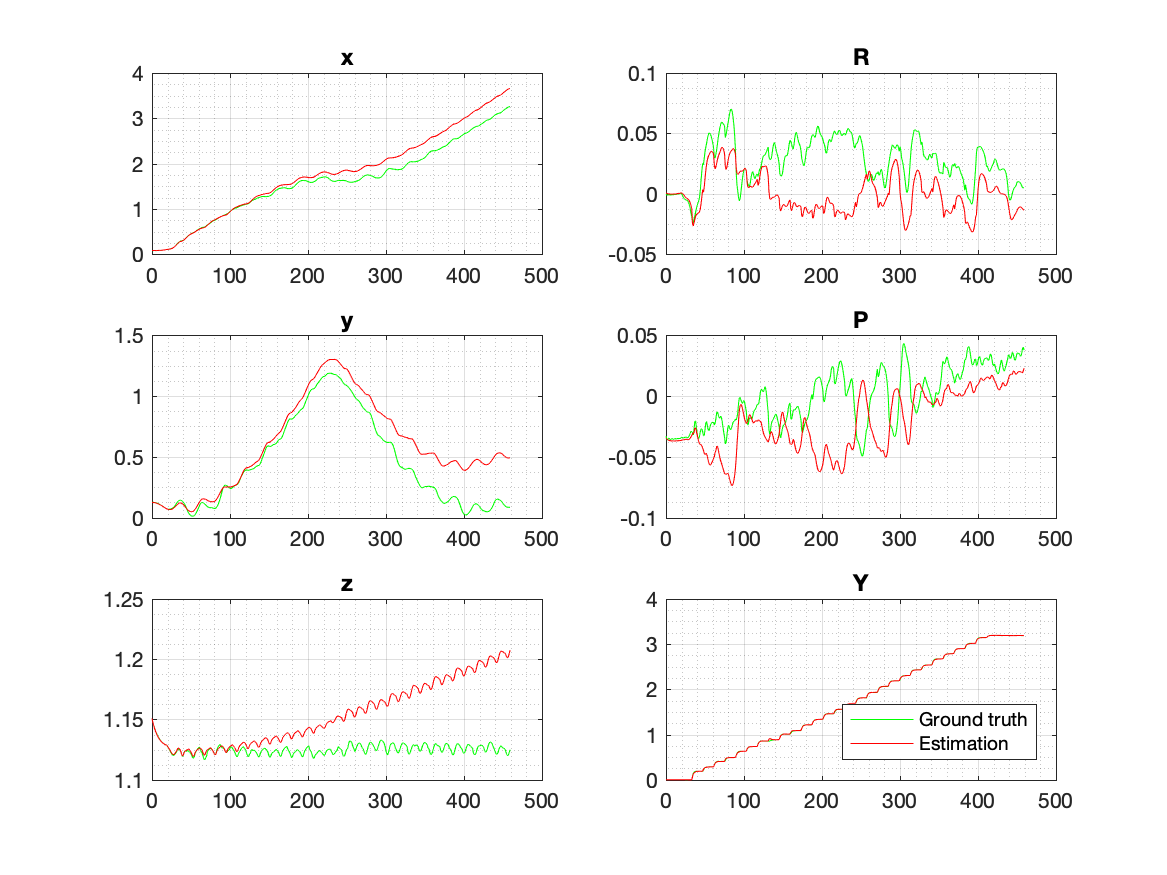
\includegraphics[width=\textwidth]{images/accelerometer.png}
    \caption{Comparison between the ground truth (in green) and the estimate (in red) of the torso
        pose when using a double integrator on the data of the accelerometer
        and the gyroscope. $x$, $y$, $z$ stands for the position
        of the torso expressed in the reference frame of the
        world. $R$, $P$, $Y$ stands for the rotations roll,
        pitch, yaw around the respective axes of the
        reference frame of the world.}
    \label{fig:comp_ground_truth_estimated_torso_accelerometer}
\end{figure}

The main reason why the method is not working is because the integration of the
linear acceleration is subject to drift, hence, the velocity term computed in
Eq. \ref{eq:velocity-accelerometer-integration} is accumulating an error
at each timestep.

\subsection{Filtering Linear Velocities}
One way to fix the problem of drift accumulation on the
integration of the acceleration is to add the linear velocity to the EKF. Nevertheless, since this
requires an observation function for the linear velocity and since
the velocity from a timestep to the following one are similar, we decided to
approximate it using the difference of the position of the robot between
two successive timesteps, which are already filtered:
\begin{equation}
    \bm{\dot{p}}_{t,k} \approx \bm{\dot{\hat{p}}}_{t,k} \approx \bm{\dot{\hat{p}}}_{t,k-1}
    = \frac{\bm{\hat{p}}_{t,k} - \bm{\hat{p}}_{t,k-1}}{T}
\end{equation}

This approximation, which has been used in Eq.
\ref{eq:position-accelerometer-integration} in our implementation,
improves the previous results
(Fig. \ref{fig:comp_ground_truth_estimated_torso_accelerometer_prevlinearvelocity}),
estimating correctly the coordinates $(x, y)^T$
and reducing the error on $z$. Even if the error on $z$ has been improved, it
does not seem to be converging like the other two coordinates.
This suggests that another approach is needed
in order to further improve the estimate.
\begin{figure}
    \centering
    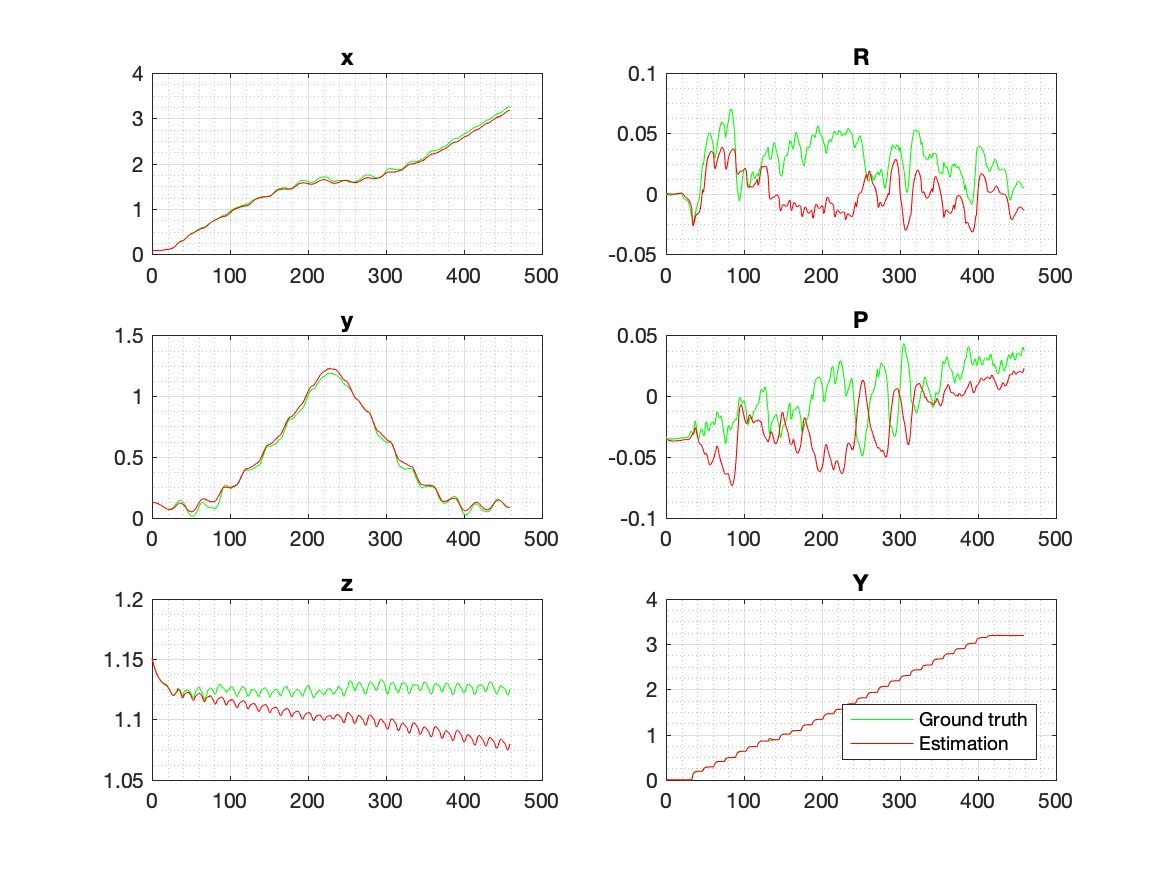
\includegraphics[width=\textwidth]{images/accelerometer_prev_linearvelocity.png}
    \caption{Comparison between the ground truth (in green) and the estimate (in red) of the torso
        pose when using a double integrator on the data of the accelerometer
        and the gyroscope. Here the velocity is approximated with the velocity
        of the previous step, which is in turn computed using the positions
        coming from the EKF. This should give an idea about what happens if the
        velocities are filtered as well. $x$, $y$, $z$ stands for the position
        of the torso expressed in the reference frame of the
        world. $R$, $P$, $Y$ stands for the rotations roll,
        pitch, yaw around the respective axes of the
        reference frame of the world.}
    \label{fig:comp_ground_truth_estimated_torso_accelerometer_prevlinearvelocity}
\end{figure}

\subsection{Trilateration}
In our third experiment we equipped the robot with a RGBD camera positioned
on top of its head and we added 6 spheres of different colors to the scene as
already explained in subsection \ref{subsec:trilateration}. The parameters of
the camera are those defined in Table \ref{table:trilateration-rgbd-params}.
All the spheres
have radius $\bar{r}=0.05$.

\begin{table}
	\centering
	\begin{tabular}{*{2}{c}}
		Camera Params. & Description \\
		\hline
		$w=512$ & width of the image \\
        $h=512$ & height of the image \\
        $\lambda=0.01 [m]$ & nearest clipping plane \\
        $\lambda_f=10.0 [m]$ & furthest clipping plane \\
        $\phi=\pi/3 [rad]$ & perspective angle \\
	\end{tabular}
	\caption{Parameters of the RGBD camera used to do trilateration.}
	\label{table:trilateration-rgbd-params}
\end{table}

We then redefined
the measurement function so that the position of the torso observed by the
robot is the one defined by Eq. \ref{eq:torso-position-trilateration}.
Fig. \ref{fig:comp-ground-truth-estimated-torso} shows the results obtained
when doing trilateration for the measurement of the position. It is
clearly possible to notice that not only the estimate of $z$ has improved with
respect to the previous experiment, but also $x$ and $y$ are closer to the
ground truth. As in the
previous experiments, the measurement of
the orientation has been computed using the gyroscope.

\begin{figure}
    \centering
    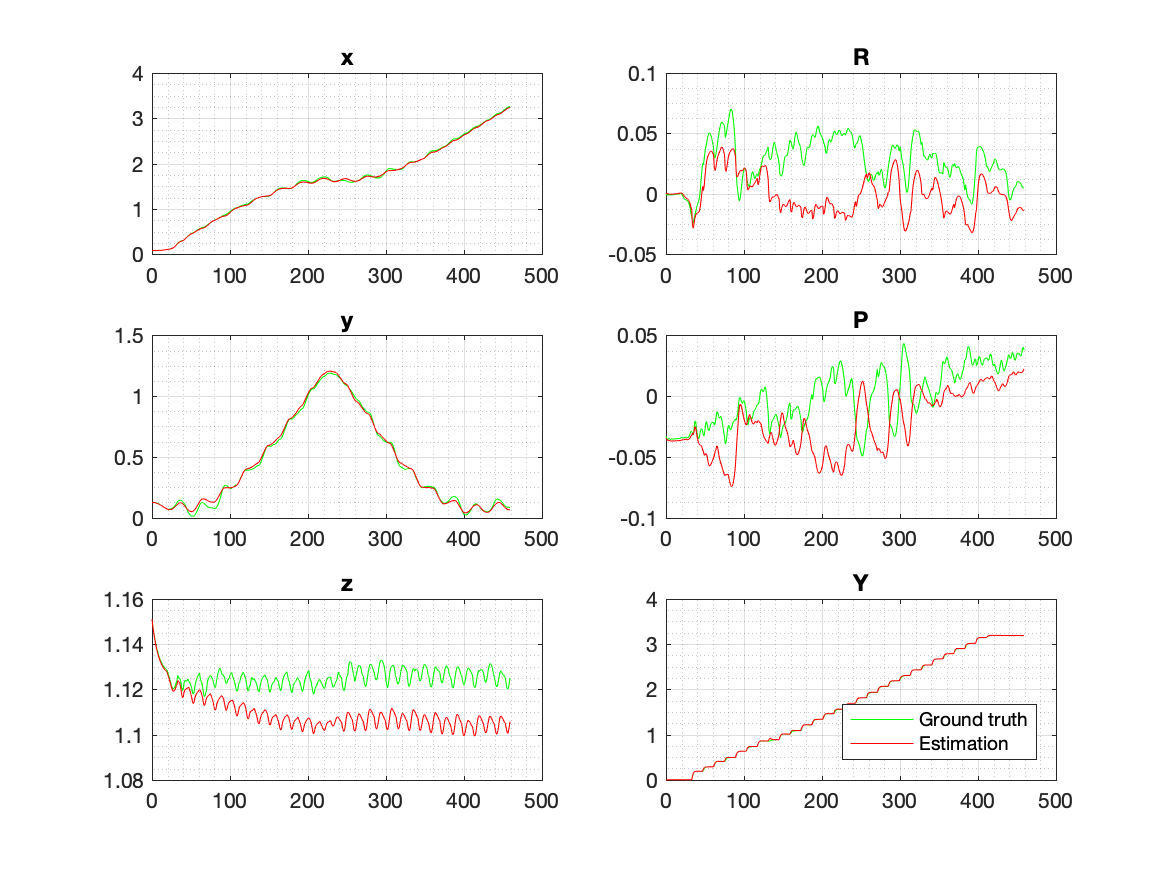
\includegraphics[width=\textwidth]{images/trilateration.png}
    \caption{Comparison between the pose of the torso estimated
        with the EKF (in red) with respect to the ground
        truth (in green) when using trilateration and the data coming
        from the gyroscope. $x$, $y$, $z$ stands for the position
        of the torso expressed in the reference frame of the
        world. $R$, $P$, $Y$ stands for the rotations roll,
        pitch, yaw around the respective axes of the
        reference frame of the world.}
    \label{fig:comp-ground-truth-estimated-torso}
\end{figure}

%\begin{figure}
%    \centering
%    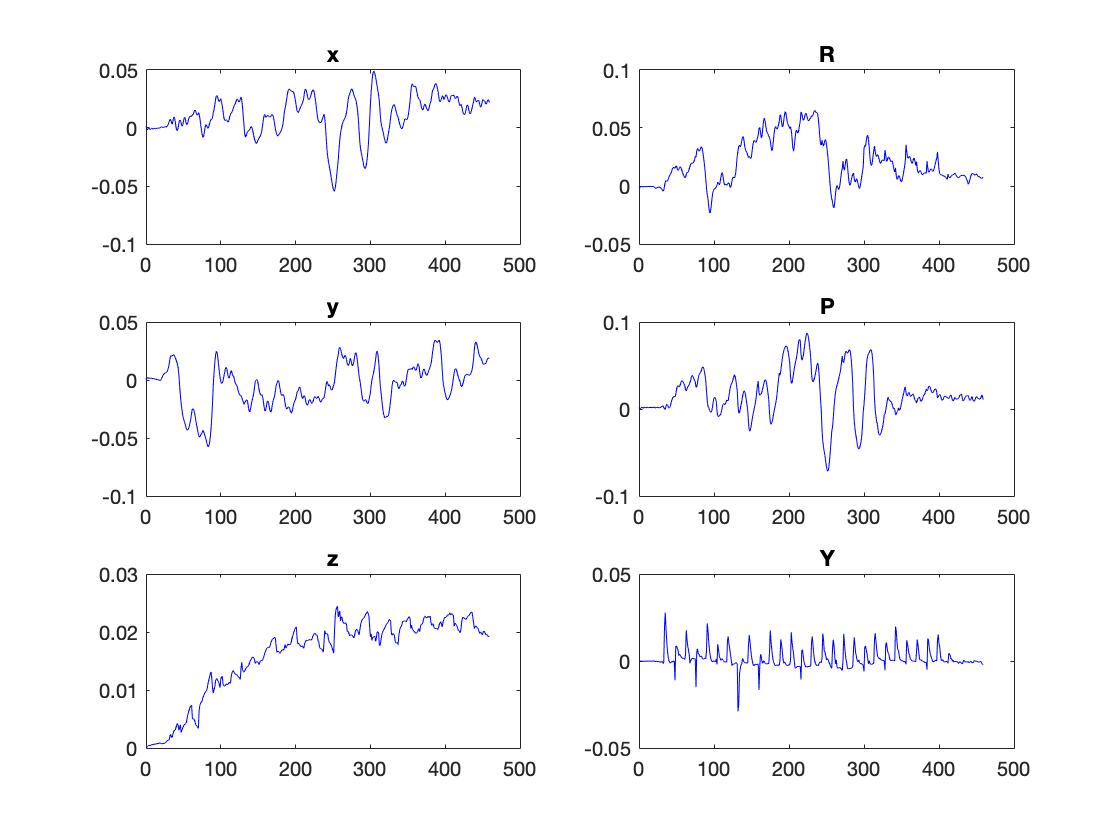
\includegraphics[width=\textwidth]{images/diff_ground_truth_estimated_torso.jpg}
%    \caption{Difference of the pose of the torso estimated
%        with the EKF with respect to the ground
%        truth. $x$, $y$, $z$ stands for the position
%        of the torso expressed in the reference frame of the
%        world. $R$, $P$, $Y$ stands for the rotations roll,
%        pitch, yaw around the respective axes of the
%        reference frame of the world.}
%    \label{fig:diff_ground_truth_estimated_torso}
%\end{figure}

\subsection{MPC Loop Closure}
Given the estimate of the pose of the torso $\bm{\hat{x}}$ we checked whether it
could be used to estimate also the position of the CoM of the robot
$\bm{\hat{p}}_{CoM}$ with respect to the world frame (Eq.
\ref{eq:pose-rf-com-world}), correctly converging to the ground truth.
The results are shown in Fig.
\ref{fig:comp_estimated_torso_com}.

We then expressed the position of the CoM
in a rotated reference frame of the support foot $\mathcal{F}_{s'}$
(as described in section \ref{section:mpc-loop-closure}) using it as a reference
signal for the MPC, without achieving the
desired behaviour. The robot, in fact, falls after a few steps even when using
a very low weight\footnote{The weight establishes the importance of the
estimate with respect to the optimal value.} in the MPC implementation. %This
%method does not improve the original implementation which considers the
%position of the CoM expressed in the reference frame of the support foot (just
%computed with forward kinematics). We think that this is due to the
%impossibility of approximating the roll and pitch angles of the support foot
%to $0$ in the C++ implementation of the HRP4 kinematics.
\begin{figure}
    \centering
    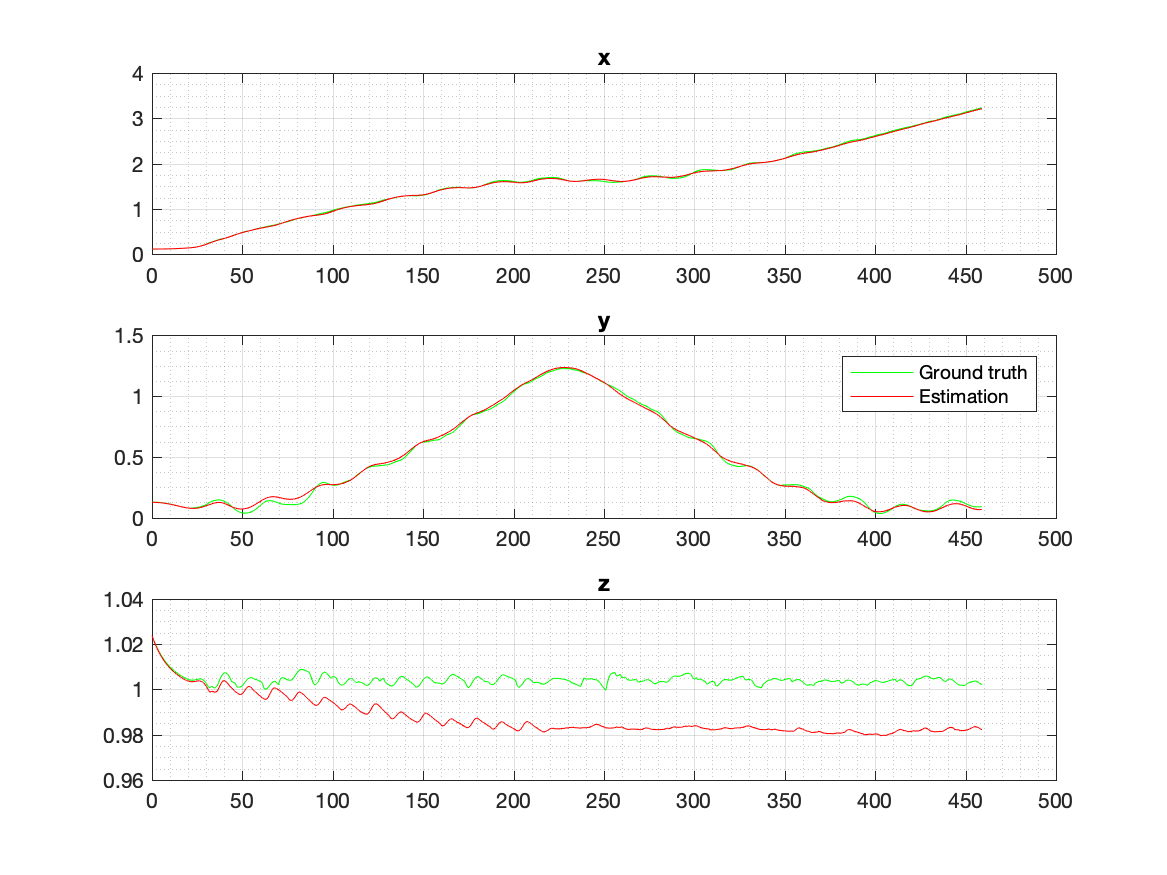
\includegraphics[width=\textwidth]{images/trilateration_com.png}
    \caption{Comparison between the estimate of the position of the CoM
        obtained with the EKF (in red) and the ground truth of the CoM
        (in green) when using trilateration and the gyroscope.
        $x$, $y$, $z$ stands for the position
        of the torso expressed in the reference frame of the
        world. $R$, $P$, $Y$ stands for the rotations roll,
        pitch, yaw around the respective axes of the
        reference frame of the world.}
    \label{fig:comp_estimated_torso_com}
\end{figure}

\subsection{Proportional Controller}
We tested the behaviour of the EKF when the robot is
performing cartesian regulation (subsection \ref{subsec:proportional_controller}).
We modeled the HRP4 as a unicycle (Equations
\ref{eq:kinematic-model-unicycle-xdot}-\ref{eq:kinematic-model-unicycle-thetadot})
and we made it move from its initial
configuration $\bm{q}_s$ to a final configuration $\bm{q}_g = (-3, 5, \cdot)^T$,
making it stop when $\left\|\bm{p}_g - \bm{\hat{p}}_t \right\| < 0.25$
in order to avoid problems due to
the oscillation of the humanoid (Fig. \ref{fig:proportional_controller_xy}).
\begin{figure}
    \centering
    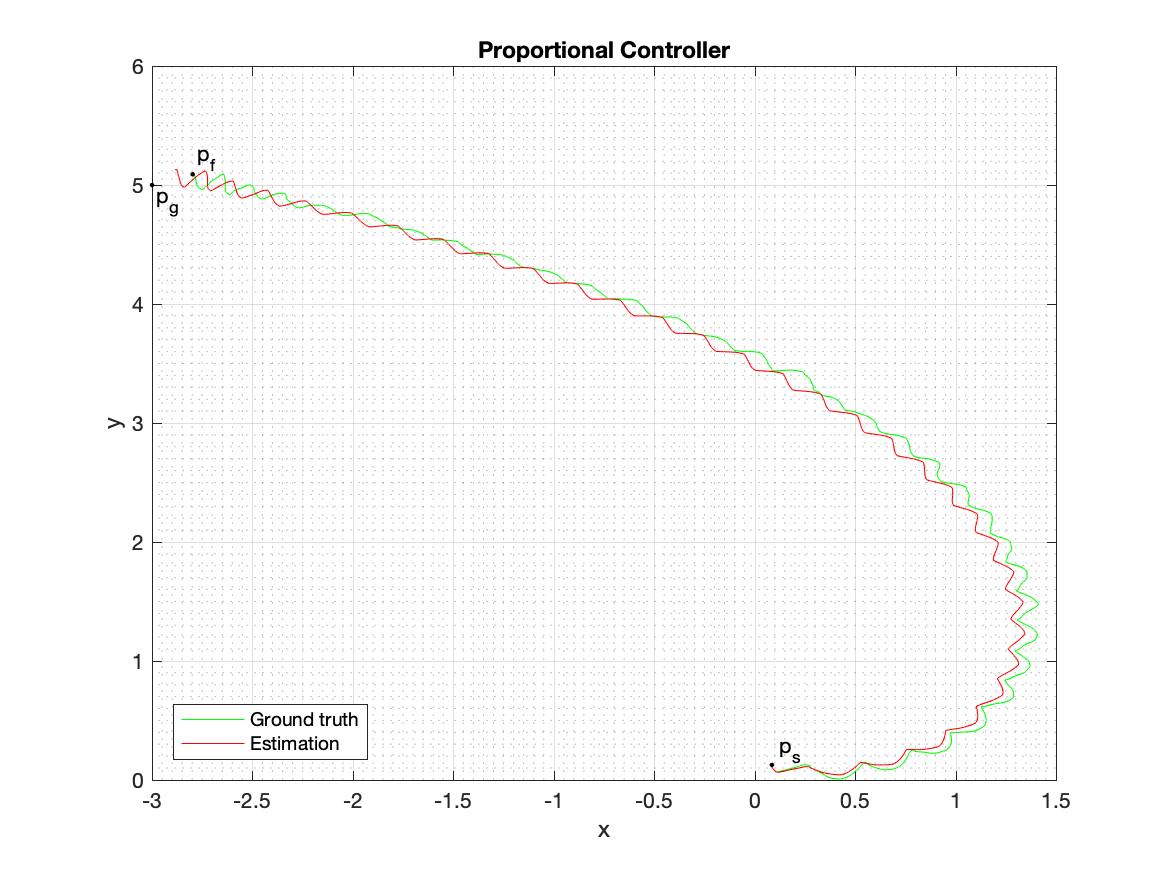
\includegraphics[width=\textwidth]{images/proportional_controller.png}
    \caption{Trajectory followed by the robot when moving to a desired configuration
        $\bm{q}_g = (-3, 5, \cdot)^T$ using the proportional controller
        described in subsection \ref{subsec:proportional_controller}.
        Here, the measurements of the Kalman filter are obtained
        using the accelerometer and the gyroscope. In green the ground truth of the coordinates $(x, y)$ of the
        robot, in red the estimate of the EKF. The robot start at the
        position $\bm{p}_s$ and it stops at the position $\bm{p}_f$. Note that,
        as explained in section \ref{subsec:proportional_controller},
        when $\left\|\bm{p}_g - \bm{\hat{p}}_t \right\| < 0.25$, $v$ are $w$ are set to 0.}
    \label{fig:proportional_controller_xy}
\end{figure}

The control law defined by Equations
\ref{eq:proportional-controller-control-law-v}-\ref{eq:proportional-controller-control-law-w},
when using gains $k_1=0.18$, $k_2=0.014$ makes the robot stop at the final
configuration $\bm{q}_f = (-2.798, 5.090, 0.98\pi)^T$, near the estimate
$\bm{\hat{q}}_f = (-2.885, 5.127, 0.979\pi)^T$ and
near the desired final configuration $\bm{q}_g$.

\subsection{Cartesian Regulation}
We then tested cartesian regulation (subsection \ref{subsec:cartesian_regulation})
on a different control law, modelling the HRP4 as in the previous experiment.
We made the robot move from its initial
configuration $\bm{q}_s$ to a final configuration $\bm{q}_g = (-2, 3.2, \cdot)^T$,
making it stop when $\left\|\bm{p}_g - \bm{\hat{p}}_t \right\| < 0.2$ as it is
possible to see from Fig. \ref{fig:cartesian_regulation_xy}.
\begin{figure}
    \centering
    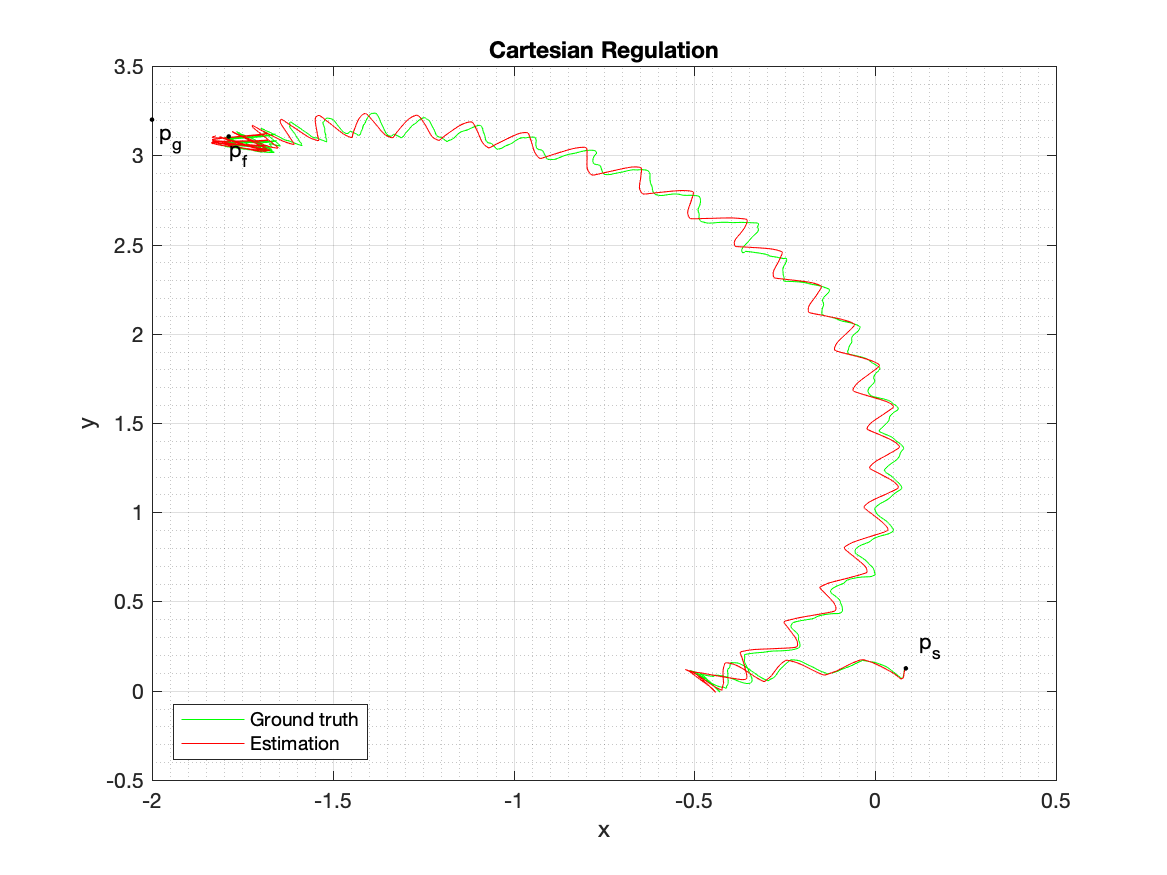
\includegraphics[width=\textwidth]{images/cartesian_regulation.png}
    \caption{Trajectory followed by the robot when moving to a desired configuration
        $\bm{q}_g = (-2, 3.2, \cdot)^T$ using the cartesian regulation task
        described in subsection \ref{subsec:cartesian_regulation}.
        Here, the measurements of the Kalman filter are obtained
        using the accelerometer and the gyroscope. In green the ground truth of the coordinates $(x, y)$ of the
        robot, in red the estimate of the EKF. The robot start at the
        position $\bm{p}_s$ and it stops at the position $\bm{p}_f$. Note that,
        as explained in section \ref{subsec:posture_regulation},
        when $\left\|\bm{p}_g - \bm{\hat{p}}_t \right\| < 0.2$, $v$ are $w$ are set to 0.}
    \label{fig:cartesian_regulation_xy}
\end{figure}

The control law defined by Equations
\ref{eq:cartesian-regulation-control-law-v}-\ref{eq:cartesian-regulation-control-law-w},
when using gains $k_1=0.07$, $k_2=0.01$ makes robot stops at the final
configuration $\bm{q}_f = (-1.788, 3.105, 1.562\pi)^T$, near the estimate
$\bm{\hat{q}}_f = (-1.823, 3.108, 1.562\pi)^T$ and
near the desired final configuration $\bm{q}_g$. It is interesting to notice
that the robot starts oscillating on the spot when it reaches a configuration
which is close to the desired one.

\subsection{Posture Regulation}
In our last experiment we tested the behaviour of the EKF when the robot is
performing posture regulation (subsection \ref{subsec:posture_regulation}).
We modeled, again, the HRP4 as a unicycle and we made it move from its initial
configuration $\bm{q}_s$ to a final configuration $\bm{q}_g = (-2.0, 3.2, \pi)^T$,
making it stop when $\delta_r < 0.2$ in order to avoid problems due to
the oscillation of the humanoid.

As it is possible to see from Figures
\ref{fig:walk_to_desired_position}-\ref{fig:walk_to_desired_position_yaw},
the robot is able to move to the desired configuration by first going
backward (keeping the same orientation) and then by simultaneously moving forward
and rotating until the desired final orientation is reached.
\begin{figure}
    \centering
    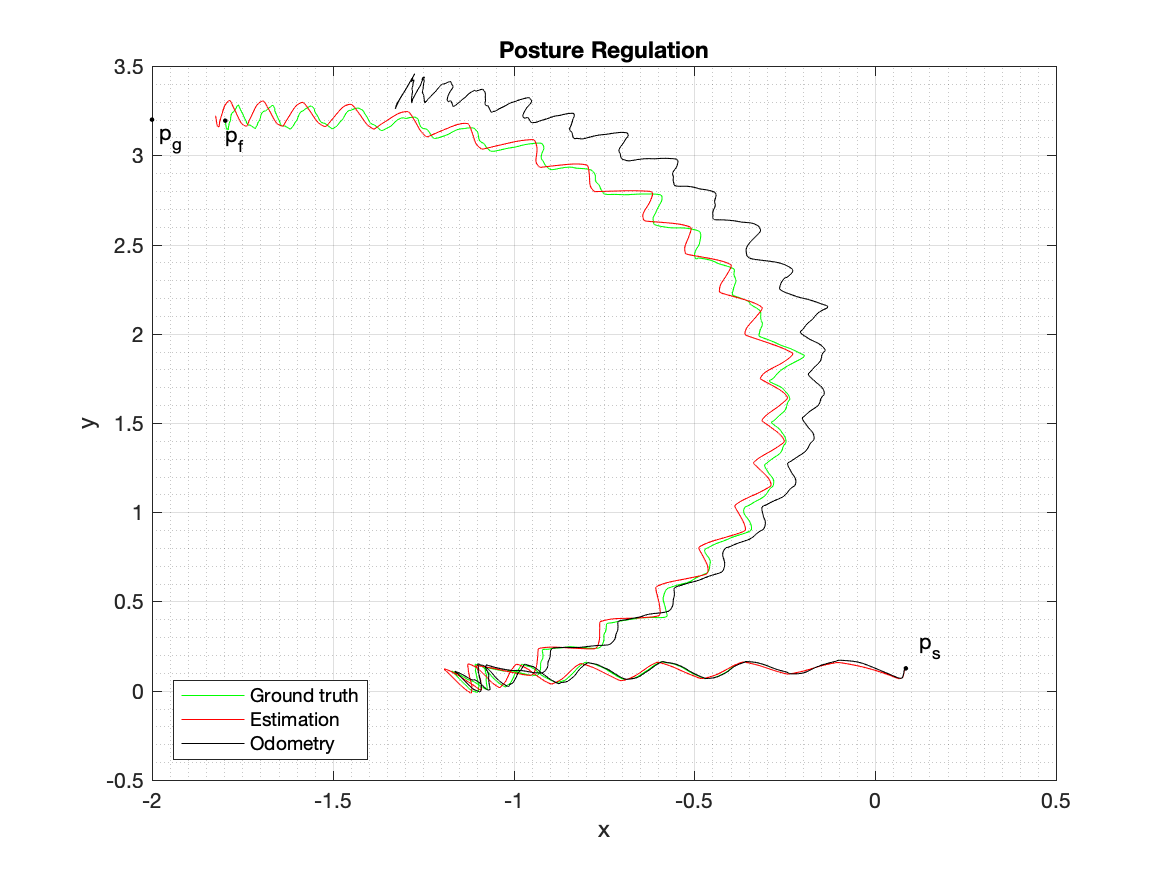
\includegraphics[width=\textwidth]{images/posture_regulation.png}
    \caption{Trajectory followed by the robot when moving to a desired configuration
        $\bm{q}_g = (-2, 3.2, \pi)$ while performing the posture regulation task
        described in subsection \ref{subsec:posture_regulation}.
        Here, the measurements of the Kalman filter are obtained
        using the accelerometer and the gyroscope. In green the ground truth of the coordinates $(x, y)$ of the
        robot, in red the estimate of the EKF, in black the odometry. The robot start at the
        position $\bm{p}_s$ and it stops at the position $\bm{p}_f$. Note that,
        as explained in section \ref{subsec:posture_regulation},
        when $\rho_r < 0.2$, $v$ are $w$ are set to 0.}
    \label{fig:walk_to_desired_position}
\end{figure}

\begin{figure}
    \centering
    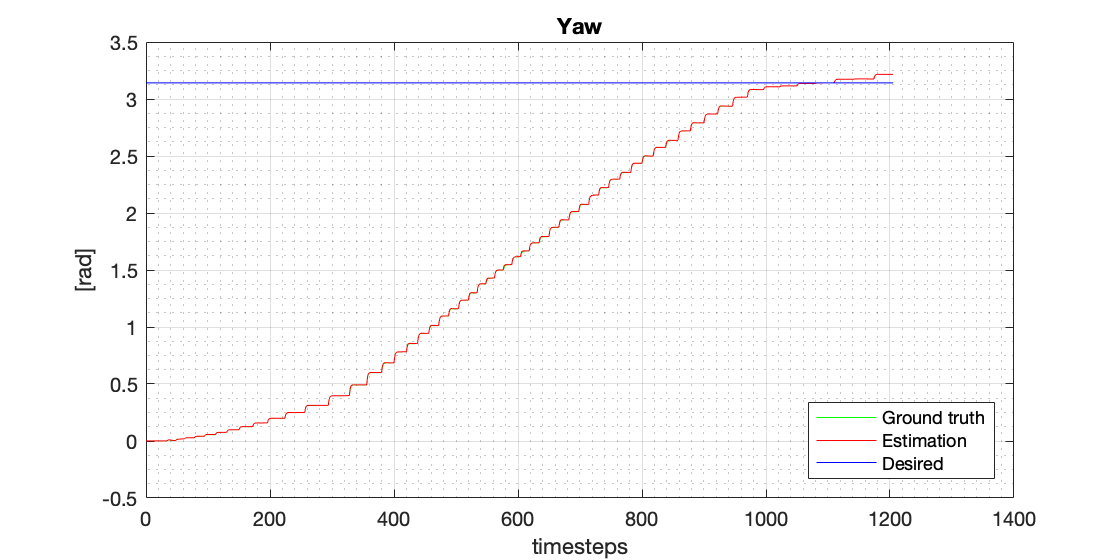
\includegraphics[width=\textwidth]{images/yaw_postureregulation.png}
    \caption{Orientation followed by the robot when moving to a desired configuration
        $\bm{q}_g = (-2, 3.2, \pi)^T$ while performing the posture regulation task
        described in subsection \ref{subsec:posture_regulation}.
        Here, the measurements of the Kalman filter are obtained
        using the accelerometer and the gyroscope. In green the ground truth of the coordinate $\theta$ of the
        robot (unicycle), in red the estimate of the EKF (note that they coincide
        for the whole path). In black the odometry, in blue the desired final orientation $\theta_g = \pi$.}
    \label{fig:walk_to_desired_position_yaw}
\end{figure}

The control law defined by Equations
\ref{eq:posture-regulation-control-law-v}-\ref{eq:posture-regulation-control-law-w},
when using gains $k_1=0.1$, $k_2=0.007$ and $k_3=0.004$,
generates the velocities $v$ and $w$ shown in Fig. \ref{fig:unicycle_velocities_posture_regulation}. The robot stops at the final
configuration $\bm{q}_f = (-1.797, 3.194, 1.024\pi)^T$, near the estimate
$\bm{\hat{q}}_f = (-1.824, 3.222, 1.024\pi)^T$ and
near the desired final configuration $\bm{q}_g$. It is interesting to notice
from the plots how the lack of the correction step (given by the exteroceptive
sensors) of the Kalman filter, namely the odometry, makes the robot move to a configuration
$(-1.282, 3.424, 0.912\pi)^T$ which is far away from the desired one.
\begin{figure}
    \centering
    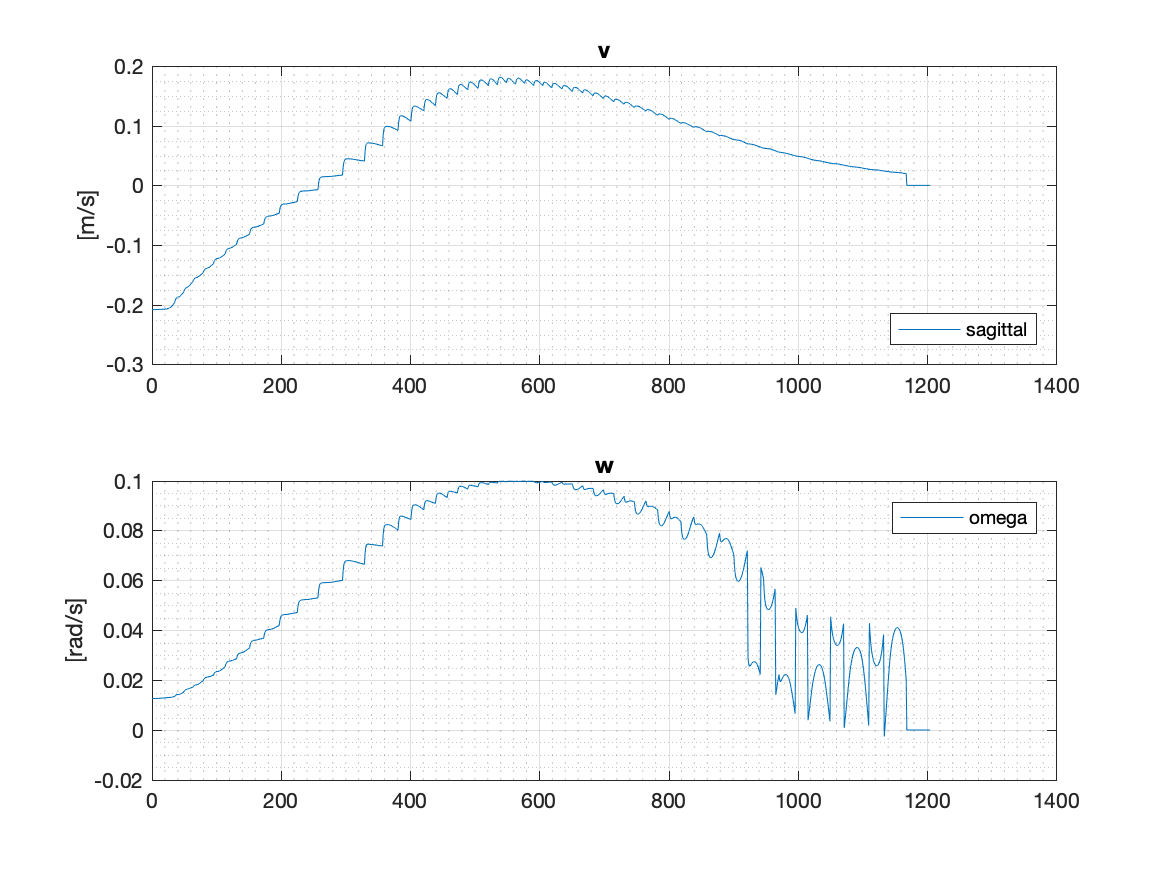
\includegraphics[width=\textwidth]{images/unicycle_velocities.png}
    \caption{Linear and angular velocity of the HRP4 while performing the
        posture regulation task described in subsection \ref{subsec:posture_regulation}.
        Note that when $\rho_r < 0.2$, $v$ are $w$ are set to 0.}
    \label{fig:unicycle_velocities_posture_regulation}
\end{figure}

\section{Conclusion}
In this project we developed an Extended Kalman Filter to localize the HRP4
humanoid robot in a V-REP environment. We equipped the robot with a gyroscope,
an accelerometer and a RGBD camera, considering different approaches in order
to make the estimate as accurate as possible. We first tested the EKF when
using only IMU measurements, not achieving convergence. We then filtered the
linear velocities of the robot improving the estimate and correctly localizing
it in the environment. Then we developed a trilateration algorithm
and used a RGBD camera further improving the estimate. We validated our
implementation on cartesian and posture regulation tasks, correctly
achieving the desired configuration. In the end we used the estimate of the
CoM of the robot to close the feedback loop of the MPC gait generator but we did not
achieved the desired behaviour, suggesting that a deeper study is needed in the
implementation of the MPC.

The behaviour of the EKF could be further improved by fusing the sensors used in
the project. Moreover, developing a proper VSLAM system could make the robot
localize in more complex environments, enabling advanced behaviours and increasing
the chances of making the MPC work correctly.

%++++++++++++++++++++++++++++++++++++++++
% References section will be created automatically
% with inclusion of "thebibliography" environment
% as it shown below. See text starting with line
% \begin{thebibliography}{99}
% Note: with this approach it is YOUR responsibility to put them in order
% of appearance.

\clearpage
\bibliography{bibliography}
\bibliographystyle{ieeetr}

%\begin{thebibliography}{99}

%\bibitem{melissinos}
%A.~C. Melissinos and J. Napolitano, \textit{Experiments in Modern Physics},
%(Academic Press, New York, 2003).

%\bibitem{Cyr}
%N.\ Cyr, M.\ T$\hat{e}$tu, and M.\ Breton,
% "All-optical microwave frequency standard: a proposal,"
%IEEE Trans.\ Instrum.\ Meas.\ \textbf{42}, 640 (1993).

%\bibitem{Wiki} \emph{Expected value},  available at
%\texttt{http://en.wikipedia.org/wiki/Expected\_value}.

%\end{thebibliography}


\end{document}
